% This is samplepaper.tex, a sample chapter demonstrating the
% LLNCS macro package for Springer Computer Science proceedings;
% Version 2.21 of 2022/01/12
%
\documentclass[runningheads]{llncs}
%
\usepackage[T1]{fontenc}
% T1 fonts will be used to generate the final print and online PDFs,
% so please use T1 fonts in your manuscript whenever possible.
% Other font encondings may result in incorrect characters.
%
\usepackage[outdir=./]{epstopdf}
\usepackage{graphicx}
\usepackage[spanish,es-noshorthands]{babel}
%\usepackage{Tikz}
\usepackage{pspicture}
% Used for displaying a sample figure. If possible, figure files should
% be included in EPS format.
%
% If you use the hyperref package, please uncomment the following two lines
% to display URLs in blue roman font according to Springer's eBook style:
%\usepackage{color}
%\renewcommand\UrlFont{\color{blue}\rmfamily}
%
\begin{document}
%

\title{Análisis Inteligente de Datos y Visualización aplicadas a la Investigación Criminal\\
Intelligent Data Analysis and Visualization applied to Criminal Investigation
\thanks{Universidad Nacional del Sur - Bahía Blanca - Argentina. Universidad Nacional de la Patagonia San Juan Bosco - Chubut - Argentina.}}
%
\titlerunning{Análisis y Visualización de Redes de Datos aplicada a la Justicia

Analysis and Visualization of Data Networks applied to Justice}
%

% If the paper title is too long for the running head, you can set
% an abbreviated paper title here
%
\author{Sebastián P. WAHLER\inst{1} \and
	Diego C. MARTÍNEZ\inst{1} \and
	Martín L. LARREA\inst{1}}
%
\authorrunning{S. Wahler, D. Martínez, M. Larrea}
% First names are abbreviated in the running head.
% If there are more than two authors, 'et al.' is used.
%
\institute{Departamento de Ciencias e Ingeniería de la Computación, Universidad Nacional del Sur, Av. Alem 1253, B8000CPB Bahía Blanca, ARGENTINA.
	\email{spwahler@ing.unp.edu.ar, dcm@cs.uns.edu.ar, mll@cs.uns.edu.ar}\\
	\url{https://cs.uns.edu.ar/}}
%

\maketitle              % typeset the header of the contribution
%
\begin{abstract}
\begin{abstract}
Se presenta un estudio de las técnicas y metodologías actuales de análisis inteligente de datos y visualización para la asistencia en la investigación criminal, a partir de los registros de actividades delictivas, sus autores y las relaciones de datos que puedan derivarse a partir de ellas. Como corolario de la investigación, se muestra el desarrollo de un módulo de software para la visualización. Es de especial interés la identificación de redes ilegales, tales como bandas delictivas o criminales para propender a una persecución penal inteligente.  

\keywords{Investigación Criminal \and Análisis Inteligente de Datos \and Redes Sociales \and Visualización.}
\end{abstract}

\renewcommand{\abstractname}{Abstract}
\begin{abstract}
A study of the current techniques and methodologies of intelligent data analysis and visualization for assistance in criminal investigation is presented, based on the records of criminal activities, their authors and the data relationships that can be derived from them. As a corollary of the investigation, the development of a software module for visualization is shown. The identification of illegal networks, such as criminal gangs, is of special interest in order to promote intelligent criminal prosecution.
	
\keywords{Criminal Investigation \and Data Analysis \and Social Networks \and Visualization.}
\end{abstract}


\end{abstract}
%
%
\section{Introducción}

En la actualidad las actividades criminales habituales en una ciudad o región van desde hurtos y robos de poca importancia, hasta otros de mayor gravedad como amenazas, cibercrimen, abusos sexuales y  homicidios. Todos ellos son registrados de diferentes formas por las fuerzas de la ley, con datos de variada precisión que incluyen usualmente la tipificación del delito, los datos en tiempo y espacio, y en muchas ocasiones los autores correspondientes.

Toda esta información respalda los procesos de investigación judicial de cada caso, pero con el transcurso del tiempo constituyen una extensa base de conocimiento sobre la cual es posible extraer valiosa información para la prevención del delito y la búsqueda de la justicia. Por ejemplo, es posible identificar relaciones entre personas de acuerdo a un análisis transitivo de eventos criminales en tiempo y espacio que sugieren la conformación de bandas delictivas. Las relaciones de amistad o conveniencia entre diversos autores de actividades criminales también puede inferirse de los registros delictivos y es de extrema relevancia para la prevención del delito y la resolución de casos inconclusos.

En este trabajo es de especial interés la aplicación de estas técnicas y tecnologías, como así también el desarrollo de un módulo de software para la visualización de los datos, utilizando los registros de actividades criminales de la Provincia de Chubut a través de la colaboración del Ministerio Público Fiscal de la provincia (parte del Poder Judicial con autonomía funcional para la investigación y persecución de conductas delictivas) y las instituciones que lo asisten.

\section{Análisis de Redes Sociales (SNA)}

Desde hace algunos pocos años, el Análisis de Redes Sociales (o SNA por sus siglas en inglés de Social Network Analysis) ha contribuido a las investigaciones criminales y a las actividades de inteligencia relacionadas.
Una red social modela individuos como nodos, vinculados entre sí por arcos o aristas que representan las relaciones entre esos individuos. El estudio de estas redes es importante porque se enfoca en la abstracción de las relaciones humanas sobre uno o más aspectos particulares ~\cite{pm2018practical}~\cite{burcher2020social}. De esta manera, las redes conforman estructuras de grafos en las cuales es posible identificar diversas propiedades, tales como la relevancia o la importancia relativa de los nodos individuales en función de las conexiones existentes o el flujo de información. Según Sage~\cite{scott2011sage} , existen cuatro pilares fundamentales del análisis de redes: el reconocimiento de la importancia de las relaciones sociales entre los individuos, la recolección y análisis de datos sobre estas relaciones, la importancia de la representación visual de estos datos y la necesidad de modelos matemáticos y computacionales que expliquen los patrones de conexión entre los individuos.

En particular, la vinculación entre el estudio de las redes sociales y la investigación criminal ha sido encarada por varios autores. A mediados de los 70 se utilizaban modelos básicos para establecer y cualificar las relaciones entre individuos o actores de un escenario particular, definiendo grafos de acuerdo a la información recolectada~\cite{harper1975application}, pero el procesamiento era mayoritariamente manual y con varias etapas de refinamiento y valoración de datos. Esta es la que según Klerk~\cite{Klerks1999TheNP} sería la primera generación de análisis de redes en criminalística. La segunda generación involucra el uso de herramientas computacionales que automatiza parte de la tarea de registro y estructuración de datos. Estas herramientas además aumentaron notoriamente la cantidad de datos que se pueden analizar, haciendo mucho más ágil su registro y consulta. La tercera y actual generación establece la definición de modelos y técnicas matemáticas para la generación de nuevo conocimiento, como la identificación de posiciones de poder e influencia o la calidad de potenciales testigos o informantes. Métricas como la centralidad de un nodo en un grafo son especialmente útiles en este escenario.

Uno de los trabajos más importantes al respecto es el de Krebs ~\cite{krebs2002mapping}, en donde se identifica una parte de la red de terroristas que fue responsable de los atentados del 11 de septiembre de 2001 en Nueva York. Aquí identifica agrupaciones de individuos que se conectan entre sí por los pilotos responsables del secuestro de las aeronaves. Otros estudios similares han sido efectivos en consecuencia ~\cite{medina2014social}~\cite{qin2005analyzing}~\cite{stollenwerk2016taking}.  Por otro lado, el análisis de redes sociales ha cobrado también interés en la investigación criminal tradicional como las estructuras de la mafia o el narcotráfico ~\cite{bouchard2013advances}~\cite{bright2015use}~\cite{giommoni2017illicit}~\cite{morselli2009hells}~\cite{morselli2010assessing}. Estudios como el de Malm ~\cite{malm2011networks} han permitido identificar roles en la cadena de suministros para la fabricación de drogas ilícitas, lo que acarrea diferentes riesgos penales para cada uno de los colaboradores. Otros estudios se enfocan en el uso del análisis de las redes sociales para otras actividades criminales, como el tráfico ilícito de arte ~\cite{bichler2013small}, el lavado de dinero ~\cite{colladon2017using}~\cite{soudijn2014using}, corrupción policial ~\cite{lauchs2011corrupt} y bandas juveniles ~\cite{mcgloin2005policy}~\cite{bichler2014magnetic}. Existen también líneas de investigación en la disciplina referente al cibercrimen ~\cite{decary2014information}~\cite{decary2012social}~\cite{decary2013reputation}. Es claro entonces que el análisis de redes sociales puede ser aplicado a un amplio rango de actividades criminales y ha demostrado modelar apropiadamente características propias de las organizaciones ilegales, asistiendo a la prevención del delito y al diseño de políticas adecuadas para enfrentar estas actividades.

Existen sin embargo algunas dificultades que requieren aún estudios intensivos. La cantidad de información que debe manejarse es enorme, en muchos casos con información incompleta, contradictoria y no menos frecuentemente incorrecta. Además, las relaciones humanas tradicionales se mezclan naturalmente con las interacciones ilícitas entre los individuos por lo que es necesario identificar apropiadamente su naturaleza y consecuencias y determinar los límites sensatos de la red social analizada. 

Actualmente los organismos estatales encargados de la Justicia y la prevención del delito cuentan con registros informatizados de las actividades criminales detectadas, así como de las etapas y eventos del subsecuente proceso penal. En particular, para este trabajo es de especial interés la información producida a tal efecto por las fuerzas policiales de la Provincia del Chubut y su Poder Judicial de la mano del Ministerio Público Fiscal (MPF). Existen decenas de miles de registros que son utilizados principalmente para la acción penal, pero que pueden ser empleados para modelar diferentes redes sociales sobre las cuales aplicar un análisis matemático y computacional en la búsqueda de nueva información. Esto permitirá conocer más sobre las actividades criminales y sus autores en la jurisdicción de esa provincia, con las particularidades propias de la información registrada digitalmente.

El análisis y exploración de estos grandes conjuntos de datos y sus relaciones debe ser asistido por técnicas y herramientas que faciliten este proceso y reduzcan la carga cognitiva que recae sobre los usuarios. En tal sentido, el área de Visualización de Información, en particular la Visualización de Grandes Conjuntos de Datos, busca asistir a los usuarios de tal manera. La aplicación de técnicas visuales para la representación de este tipo de información no es nueva ~\cite{xu2005criminal}~\cite{feng2019big}~\cite{mathew2021criminal}. También es importante el estudio de las tareas e interacciones que la visualización debe soportar ~\cite{chen2005visualization}, ya que son estas interacciones las que facilitan la exploración de la visualización de información.


\section{Marco de Trabajo - Ministerio Público Fiscal del Chubut}
En el marco de trabajo se ha optado por investigar en base al análisis criminal de redes delictivas en el Ministerio Público Fiscal del Chubut ~\cite{MPFChubutPaginaWeb}, perteneciente al Poder Judicial de la provincia.
Coirón es el sistema informático que colabora con la administración del flujo de casos ingresados al Ministerio Público Fiscal del Chubut. Es una herramienta que permite registrar, comunicar y gestionar las actividades, trámites y actuaciones que se realizan para un caso penal, desde la denuncia hasta su finalización. 
Como herramienta de registro construye una base de datos con el historial de cada caso, así como de las personas involucradas y de los responsables de la gestión en cada oficina. Como herramienta de comunicación, agrupa la información, entrecruza las relaciones, identifica pertenencias y vinculaciones entre casos, personas, sus antecedentes y sus lazos. Como herramienta de gestión administra el flujo de casos y el trabajo de los integrantes de las oficinas responsables de los mismos. Permite planificar, organizar, coordinar y controlar el flujo de trabajo afín a cada caso y la sumatoria de ellos.
Ha sido desarrollado a medida de las necesidades del Ministerio Público Fiscal del Chubut, tomando como base el Código Procesal Penal vigente y adaptado a los lineamientos estratégicos de diseño y gestión de Oficinas Fiscales definidos por la Procuración General. Su progreso, mantenimiento y mejora continua está a cargo del Equipo de Desarrollo del Departamento de Informática del Área de Planificación y Control de Gestión de la Procuración General. Una vez registrada toda la información relacionada a un hecho, y con ayuda de herramientas y vinculaciones con otros sistemas, se pueden obtener salidas que permiten llevar adelante la investigación de un caso o de un conjunto de hechos con características comunes.

Actualmente nos encontramos trabajando en la incorporación de herramientas de visualización de información que permitirán ver en modo gráfico lo que hoy se muestra en grillas, y listados, potenciando el análisis que realizarán luego los especialistas. Desde el análisis criminal, se puede realizar un perfilamiento relacional para la persecución penal, a través de la vinculación de "compañeros" de delitos y de redes sociales; a fin de identificar si forman parte de una banda o alguna organización criminal mayor~\cite{rua2020perspectiva}. En este sentido los analistas de redes sociales utilizan dos tipos de herramientas matemáticas para representar información sobre los patrones de relaciones entre actores sociales: matrices y grafos, de gran ayuda visual cuando se trabaja con una gran cantidad de registros.

Existen muchas variaciones en los grafos, pero todos ellos comparten la característica común del uso de un círculo etiquetado para cada actor en la población que describimos y segmentos de línea entre pares de actores para representar el hecho que existe un vínculo entre ellos. Se denomina "Grupo de Pertenencia" en el Sistema Coirón a la relación directa que existe entre un individuo dentro del universo de personas cargadas como actores de delitos (roles: denunciado, sospechoso o imputado) y otros individuos del mismo universo, con los cuales existan uno o más casos penales en común.

Crear un módulo de software "Red de Grupos de Pertenencia" donde se muestre gráficamente las relaciones entre las personas involucradas en los casos penales es el objetivo principal de esta investigación. No sólo enfocarse en el grupo de pertenencia de una persona en particular, sino que mediante una visualización y con diversos filtros de búsqueda, se logre mostrar gráficamente las relaciones entre un determinado grupo de personas y de esta manera poder inferir la conformación de posibles bandas delictivas.

La idea central es reflejar de manera gráfica, mediante un Grafo, los grupos de pertenencia. Dentro del mismo se le llamará nodo a cada círculo, y representa a una persona (con los roles ya mencionados: imputado, sospechoso o denunciado) involucrada en dos o más casos penales. Existe un gran cúmulo de personas en el sistema con sólo un caso con rol de denunciado, por esa razón se los excluye del universo a analizar, no obstante podrían ser parte del dataset a visualizar si alguno/s de ellos se encuentran relacionados con otros nodos del primer grupo. El tamaño del nodo posee una relación directa con la cantidad de casos penales en los que se encuentre involucrada la persona. Cuanto mayor sea el tamaño del nodo en más cantidad de casos penales estará involucrado.

Los segmentos de líneas entre pares de nodos, vinculan a las personas entre sí y representan el o los casos que tienen en común. El grosor de la vinculación será directamente proporcional a la cantidad de casos en común entre un par de personas. Hay nodos que se encontrarán aislados en el grafo, esto no significa que no estén involucrados en casos, sino que quizás no existan relaciones para el filtro de búsqueda que se utilice en esa vista en particular.

Supongamos que una persona "A" se encuentra asociada a 8 casos penales, una persona "B" a 4 y una persona "C" a 2 casos. Agreguemos que las personas "A" y "B" se encuentran relacionadas entre sí, por estar en 3 casos en común (casos 1, 2 y 3). Por otro lado las personas "A" y "C" también se encuentran relacionadas, por tener un caso en común (caso 4).  Una representación gráfica de dicha situación se muestra en la Figura \ref{fig:grafode2}, y puede observarse el doble de tamaño entre el nodo "A" y el nodo "B", representando justamente la diferencia de casos entre ambos nodos (8 y 4 casos). También se ve a simple vista el grosor del enlace entre "A" y "B" tres veces más grande que el enlace entre "A" y "C" (3 casos en común entre el primer par de nodos, y sólo un caso para el último par de nodos mencionado). 
%\vspace{-20pt}
\begin{figure}
	\centering
	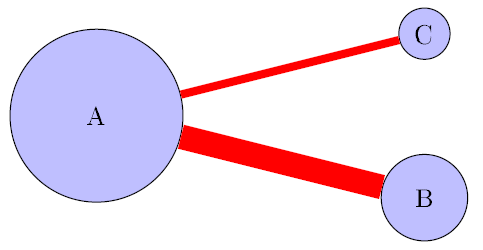
\includegraphics[width=0.3\linewidth]{grafo-ejemplo.png}
	\caption{Ejemplo de relación entre tres personas.} 
	\label{fig:grafode2}
\end{figure}
\vspace{-25pt}
%\begin{figure}
%	\centering
%	\tikzstyle{nodoA}= [circle,fill=blue!25,minimum size=60pt]
%	\tikzstyle{nodoB}=[circle,fill=blue!25,minimum size=30pt]
%	\tikzstyle{nodoC}=[circle,fill=blue!25,minimum size=15pt]
%	\begin{center}
%		\begin{tikzpicture}[scale=1.0]
%			\node[nodoA][draw] (1) at (0,6) {A};
%			\node[nodoB][draw] (2) at (4,5) {B};
%			\node[nodoC][draw] (3) at (4,7) {C};
%			%
%			\draw [line width=3.0mm, red ] (1) -- (2);
%			\draw [line width=1.0mm, red ] (1) -- (3);
%		\end{tikzpicture}
%	\caption{Ejemplo de relación entre tres personas.} 
%	\label{fig:grafode2}
%	\end{center}
%\end{figure}

\section{Descripción general de los Datos}
En esta sección, describimos nuestro conjunto de datos de casos penales y la red de personas asociada, así como algunas características interesantes que se han de mencionar.
\subsubsection{Dataset de Delitos}
Nuestro conjunto de datos consta de casos penales, actuaciones (bitácora de eventos del proceso penal), delitos, personas, elementos (denunciados y secuestrados), todos ellos relacionados; entre octubre de 2006 y mayo de 2022 en la Circunscripción Judicial de Trelew - Chubut. Este conjunto de datos incluye lugares (relativos a personas y a hechos delictivos), fechas, estados procesales de los casos y las personas, como así también los vínculos entre todos los conjuntos mencionados. En el Cuadro \ref{tab:TotalizadoresGenerales}, resumimos algunas de las características más importantes del conjunto de datos.
\vspace{-10pt}
\begin{table}
	\centering
	\label{tab:TotalizadoresGenerales}
	\begin{tabular}{|l|r|}
		\hline
		\textbf{Característica} &  \textbf{Cantidad total} \\
		\hline
		Casos &  105586 \\
		\hline
		Personas &  132950 \\
		\hline
		Personas en Casos &  183348 \\
		\hline
		Delitos &  113010 \\
		\hline
		Nodos &  33178 \\
		\hline
		Enlaces &  16964 \\
		\hline
		Relaciones Nodos/Enlaces &  60513 \\
		\hline
	\end{tabular}
	\vspace{10pt}
	\caption{Totalizadores del conjunto de datos generales}
\end{table}
\vspace{-10pt}
\subsubsection{Propiedades de la red}
A partir de los datos de los casos penales, pudimos construir la red de Grupos de Pertenencia. En esta red, se eliminan los nodos de aquellas personas cuyos roles no sean referidos a actores delictivos, como ser: denunciantes, víctimas, damnificados, etc. En la Figura \ref{fig:grafocompleto} se muestra una visualización de la red. En la misma se puede observar un grafo compuesto de más de 30000 personas con más Casos Penales registrados en el Sistema de Gestión Coirón (con los siguientes criterios: involucradas en más de un caso con rol de imputado, sospechoso o denunciado; se incluyen personas fallecidas, menores y personas jurídicas). Se visualizan además en la figura todas las relaciones que existen entre esas personas y sus grupos de pertenencia.
\vspace{-10pt}
\begin{figure}
	\centering
	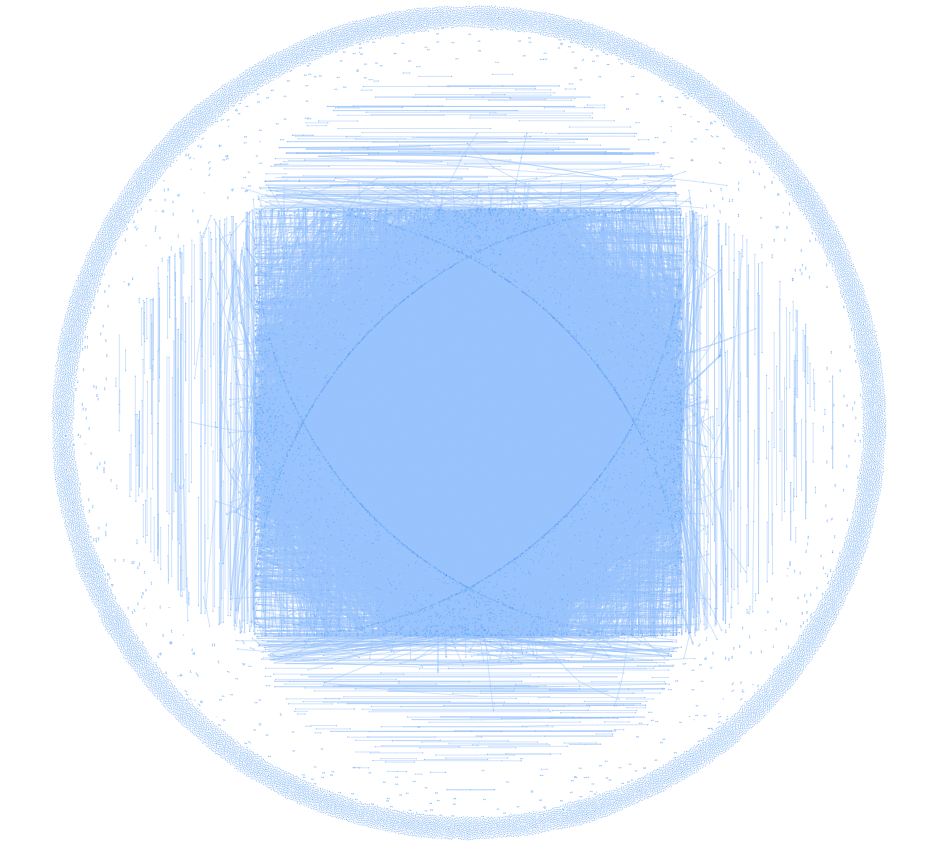
\includegraphics[width=0.4\linewidth]{grafo-30000-completo.png}
	\caption{Más de 30000 personas con más casos y sus relaciones.} 
	\label{fig:grafocompleto}
\end{figure}
\vspace{-10pt}
A los sentidos prácticos de la investigación penal, una visualización con tantos nodos y relaciones no es representativa ni conduce a ningún tipo de detección de bandas delictivas, pero es un claro ejemplo del universo de datos que se disponen en el dataset utilizado, como así también la potencia de la herramienta de visualización. En la Figura \ref{fig:grafosCompletos} se pueden observar ejemplos en los que se han tomado en cuenta los grupos de pertenencia de cada nodo a mostrar, es decir que se visualizan las personas con sus grupos de pertenencias particulares (según parámetros de búsqueda seleccionados). En la imagen (a) se muestran 10000 personas, en (b) 1000 y en (c) 100 personas con más casos y sus grupos de pertenencia relacionados.
\vspace{-10pt}
\begin{figure}[htbp]
	\centering
	\subfigure[Top 10000.]{
		\begin{minipage}[t]{0.33\linewidth}
			\centering
			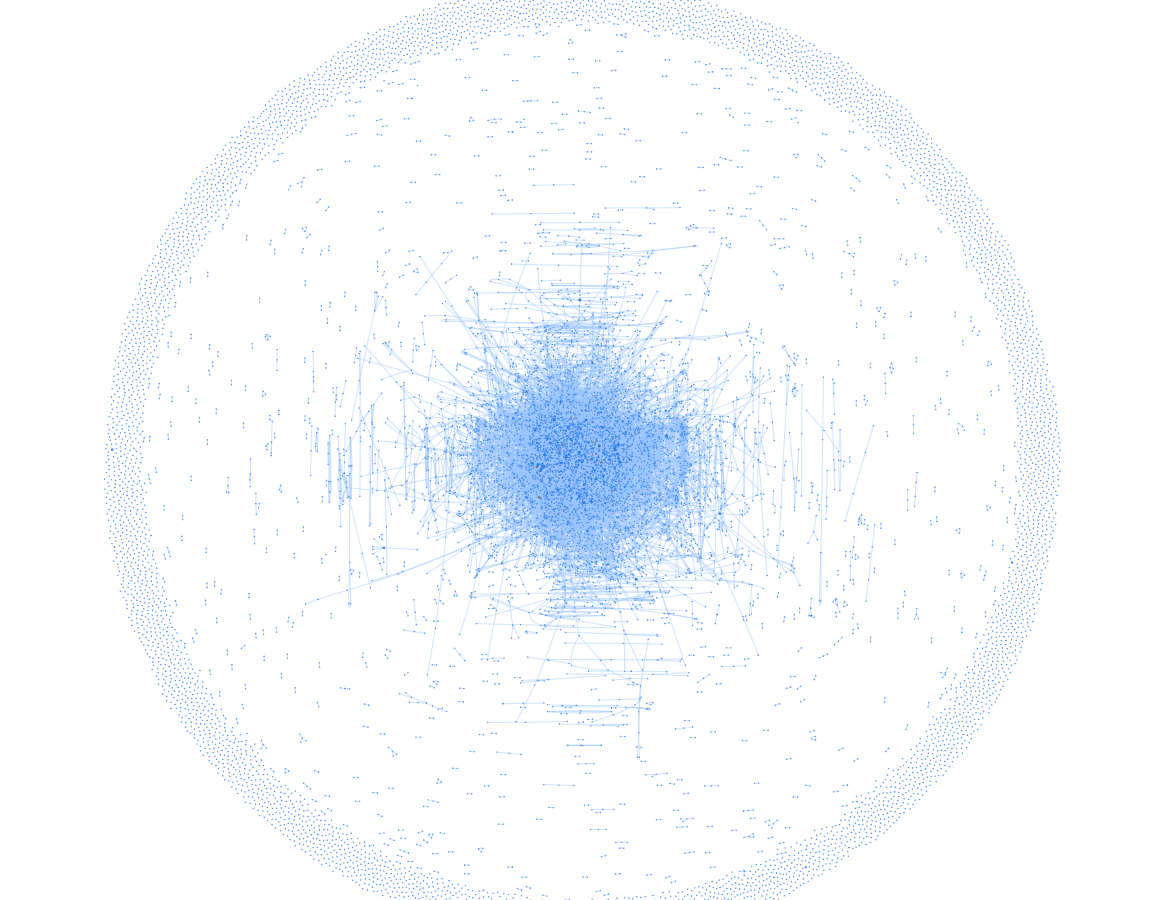
\includegraphics[width=1in]{grafo-10000-completo.png}
			%\caption{fig1}
		\end{minipage}%
	}%
	\subfigure[Top 1000.]{
		\begin{minipage}[t]{0.33\linewidth}
			\centering
			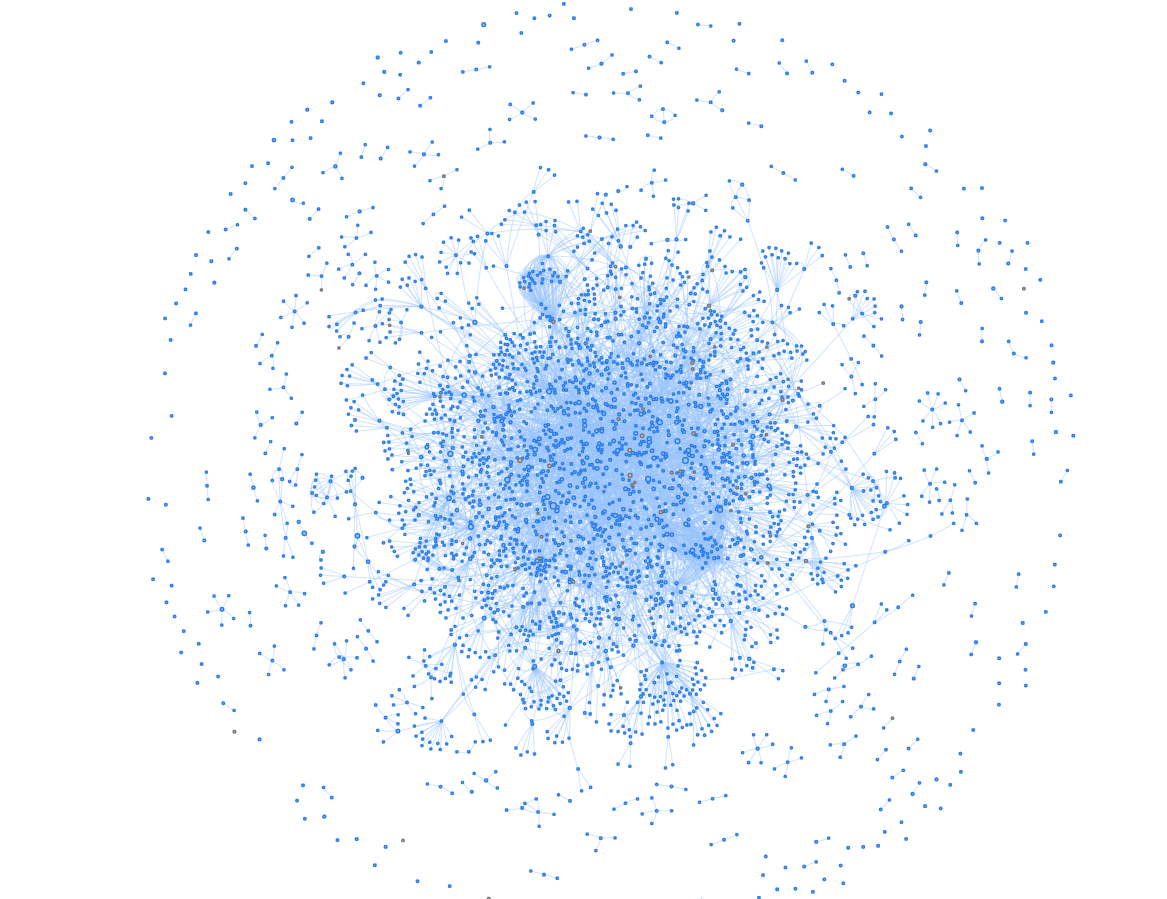
\includegraphics[width=1in]{grafo-1000-completo.png}
			%\caption{fig2}
		\end{minipage}%
	}%
	\subfigure[Top 100.]{
		\begin{minipage}[t]{0.33\linewidth}
			\centering
			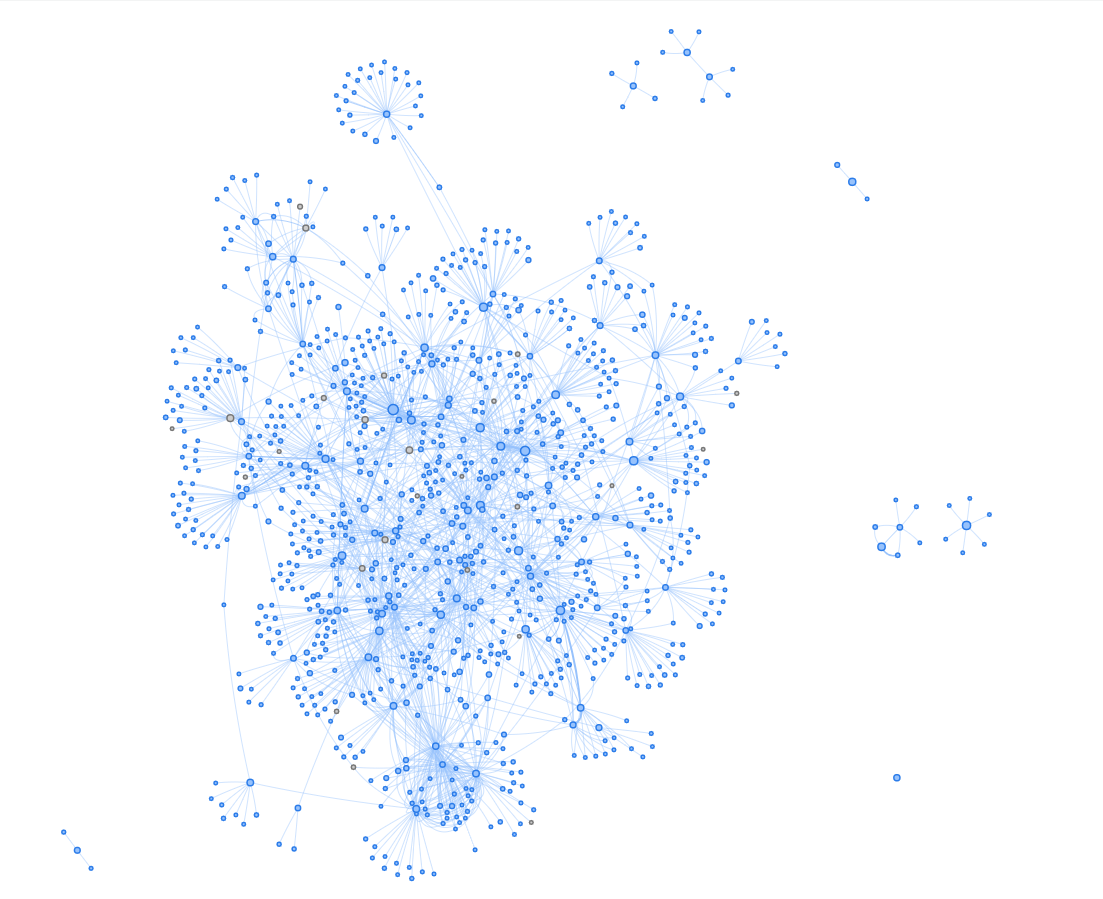
\includegraphics[width=1in]{grafo-100-completo.png}
			%\caption{fig3}
		\end{minipage}
	}%
	\centering
	\caption{ Personas en más casos, con la inclusión de sus grupos de pertenencia particulares.}
	\label{fig:grafosCompletos}
\end{figure}
\vspace{-10pt}
Al analizar la composición de la red obtenida podemos observar las relaciones que existen entre los nodos y como se "equilibra" el grafo, haciendo que aquellos nodos con pocas o nulas relaciones queden en la periferia de la gráfica. Sumado a ello también es apreciable la medida de centralidad de aquellos nodos que son rodeados por sus relacionados. Una aproximación más clara para denotar la medida de centralidad puede verse reflejada en la Figura \ref{fig:grafoTop10}, en donde se visualiza sólo las 10 personas con más Casos y sus grupos de pertenencia. Claramente esos 10 nodos principales quedan rodeados de sus grupos de pertenencia y se pueden observar transitividades entre ellos a través de nodos que conforman parte del grupo de pertenencia de más de un nodo principal.
\vspace{-10pt}
\begin{figure}
	\centering
	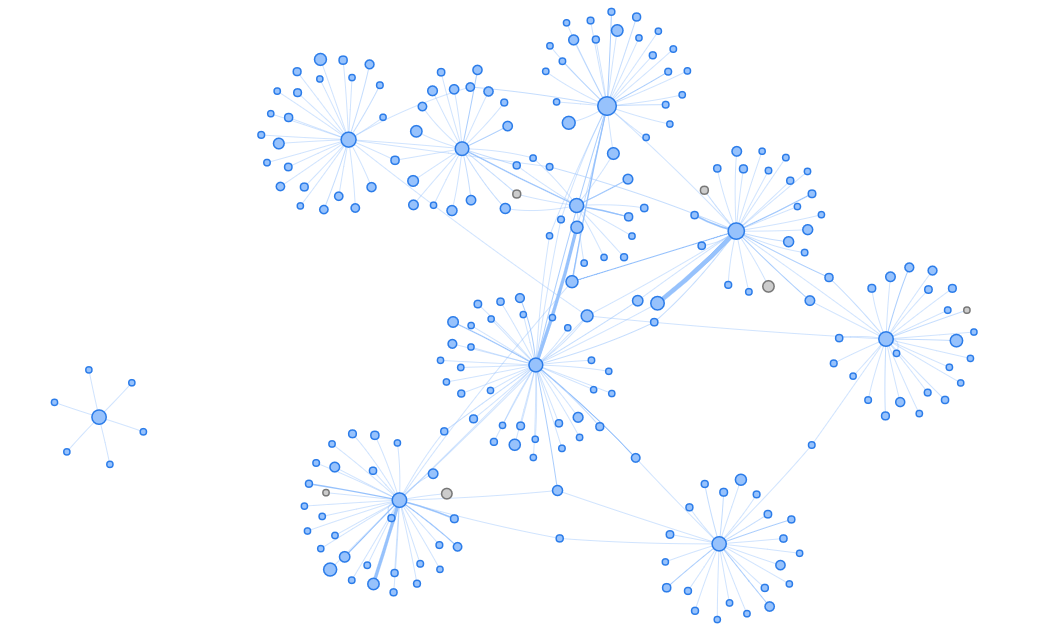
\includegraphics[width=0.5\linewidth]{grafo-10-completo.png}
	\caption{10 personas con más casos en Coirón, con sus relaciones} 
	\label{fig:grafoTop10}
\end{figure}
\vspace{-20pt}
\subsubsection{Centralidad de Grado} La centralidad de grado es una de las medidas más simples de centralidad. En esta se mide el número de enlaces o conexiones que tiene un nodo con los demás nodos pertenecientes a un grafo. Cuando se aplica un análisis de este tipo pueden determinarse diferentes medidas. Por ejemplo, en redes sociales podemos medir el grado de entrada de un nodo como la popularidad o preferencia que posea y la salida definirla como un indicador de sociabilidad. En nuestro caso de estudio, los miembros de las bandas delictivas modifican dinámicamente sus relaciones con otros miembros de la red, lo que resulta en un cambio de su rol e importancia. Una serie de medidas de centralidad de grado pueden ayudar a identificar estos cambios. Estas estadísticas se pueden utilizar para filtrar la vista de la red en función del valor de un nodo específico y resaltar su posición dentro de la red. El grado de centralidad en nuestro grafo se definirá entonces como el número de enlaces directos que tiene un delincuente. Un nodo con un alto grado puede verse como un "centro", un nodo activo e importante en la red~\cite{carley2006destabilization}.
\vspace{-10pt}
\subsubsection{Transitividad} El coeficiente de agrupamiento (transitividad) de un gráfico mide el grado de conexión de una red. Altos coeficientes de agrupamiento significan la presencia de un alto número de triángulos en la red. Es bien conocido en la bibliografía~\cite{wasserman1994social} que las redes sociales muestran valores altos del coeficiente de agrupamiento cuando reflejan la estructura social subyacente de los contactos entre amigos/conocidos. Además, los valores altos del coeficiente de agrupamiento local se consideran un indicador confiable de los nodos cuyos vecinos están muy bien conectados y entre los cuales puede fluir una cantidad sustancial de información.
\subsubsection{Desarrollo de la Visualización}
\todo{hablar de vis.js, quizás agregar algo de código}

Para llevar a cabo la visualización del conjunto de datos obtenidos del análisis inteligente anteriormente descripto, se utilizó Vis.js ~\cite{ref_visjs}, una biblioteca o librería de visualización dinámica basada en lenguaje Javascript. La misma está diseñada para que sea fácil de usar, para manejar grandes cantidades de datos dinámicos y para permitir la manipulación y la interacción con los datos. La biblioteca consta de los componentes DataSet, Timeline, Network, Graph2d y Graph3d.
En nuestro caso particular utilizamos el componente "Network", que permite mostrar redes en grafos. La visualización es fácil de usar y admite formas, estilos, colores, tamaños, imágenes, etc. La visualización de la red funciona sin problemas en cualquier navegador moderno para hasta unos pocos miles de nodos y bordes. Para manejar una mayor cantidad de nodos, Network tiene soporte de agrupamiento. La red utiliza un lienzo HTML para la representación.



\paragraph{Sample Heading (Fourth Level)}
The contribution should contain no more than four levels of
headings. Table~\ref{tab1} gives a summary of all heading levels.

\begin{table}
\caption{Table captions should be placed above the
tables.}\label{tab1}
\begin{tabular}{|l|l|l|}
\hline
Heading level &  Example & Font size and style\\
\hline
Title (centered) &  {\Large\bfseries Lecture Notes} & 14 point, bold\\
1st-level heading &  {\large\bfseries 1 Introduction} & 12 point, bold\\
2nd-level heading & {\bfseries 2.1 Printing Area} & 10 point, bold\\
3rd-level heading & {\bfseries Run-in Heading in Bold.} Text follows & 10 point, bold\\
4th-level heading & {\itshape Lowest Level Heading.} Text follows & 10 point, italic\\
\hline
\end{tabular}
\end{table}


\noindent Displayed equations are centered and set on a separate
line.
\begin{equation}
x + y = z
\end{equation}
Please try to avoid rasterized images for line-art diagrams and
schemas. Whenever possible, use vector graphics instead (see
Fig.~\ref{fig1}).

\begin{figure}
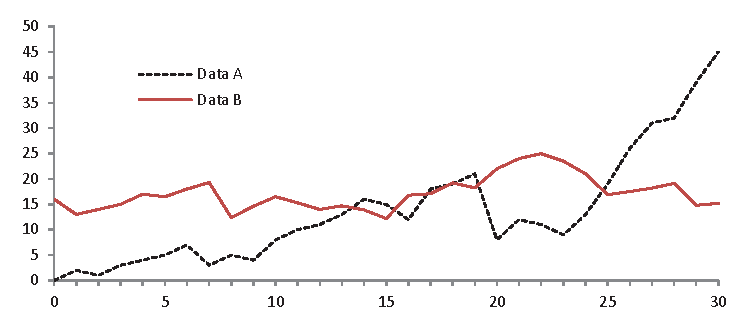
\includegraphics[width=\textwidth]{fig1.eps}
\caption{A figure caption is always placed below the illustration.
Please note that short captions are centered, while long ones are
justified by the macro package automatically.} \label{fig1}
\end{figure}

\begin{theorem}
This is a sample theorem. The run-in heading is set in bold, while
the following text appears in italics. Definitions, lemmas,
propositions, and corollaries are styled the same way.
\end{theorem}
%
% the environments 'definition', 'lemma', 'proposition', 'corollary',
% 'remark', and 'example' are defined in the LLNCS documentclass as well.
%
\begin{proof}
Proofs, examples, and remarks have the initial word in italics,
while the following text appears in normal font.
\end{proof}
For citations of references, we prefer the use of square brackets
and consecutive numbers. Citations using labels or the author/year
convention are also acceptable. The following bibliography provides
a sample reference list with entries for journal
articles~\cite{ref_article1}, an LNCS chapter~\cite{ref_lncs1}, a
book~\cite{ref_book1}, proceedings without editors~\cite{ref_proc1},
and a homepage~\cite{ref_url1}. Multiple citations are grouped
\cite{ref_article1,ref_lncs1,ref_book1},
\cite{ref_article1,ref_book1,ref_proc1,ref_url1}.

\subsubsection{Acknowledgements} Please place your acknowledgments at
the end of the paper, preceded by an unnumbered run-in heading (i.e.
3rd-level heading).

%
% ---- Bibliography ----
%
% BibTeX users should specify bibliography style 'splncs04'.
% References will then be sorted and formatted in the correct style.
%
% \bibliographystyle{splncs04}
% \bibliography{bibliografia}
%
\renewcommand{\refname}{Referencias Bibliográficas}
\begin{thebibliography}{8}
\bibitem{ref_article1}
Finckenauer JO. Problems of definition: What is organized crime? Trends in Organized Crime. 2005; 8(3):63–83. \url{https://doi.org/10.1007/s12117-005-1038-4}
\bibitem{ref_article2}
Krishna Raj P.M.Ankith MohanK.G. Srinivasa. Practical Social Network Analysis with Python. Springer, 2018. ISBN: 978-3-319-96746-2.
\bibitem{ref_article3}
Burcher, Morgan. Social Network Analysis and Law Enforcement: Applications for Intelligence Analysis. Serie Crime Prevention and Security Management, 2020. ISBN 978-3-030-47770-7
\bibitem{ref_article4}
L.C. Freeman, The SAGE handbook of social network analysis, eds. J. Scott, P.J. Carrington, SAGE Publications Ltd., 2011.
\bibitem{ref_article5}
W.R. Harper, D.H. Harris, The application of link analysis to police intelligence. Hum. Factors 17(2), 157–164 (1975).
\bibitem{ref_article6}
P. Klerks, The network paradigm applied to criminal organisations: theoretical nitpicking or relevant doctrine for investigators? Recent developments in the Netherlands. Connections 24(3), 53–65 (1999)
\bibitem{ref_article7}
V. Krebs, Mapping networks of terrorist cells. Connections 24(3), 43–52 (2002)
\bibitem{ref_article8}
R.M. Medina, Social network analysis: a case study of the Islamist terrorist network. Secur. J. 27(1), 97–121 (2014)
\bibitem{ref_article9}
J. Qin, J.J. Xu, D. Hu, M. Sageman, H. Chen, Analyzing terrorist networks: a case study of the global jihad. Lect. Notes Comput. Sci. 3495, 287–304 (2005)
\bibitem{ref_article10}
E. Stollenwerk, T. Dörfler, J. Schibberges, Taking a new perspective: mapping the Al Qaeda network through the eyes of the UN Security Council. Terror. Political Violence 28(5), 950–970  (2016)
\bibitem{ref_article11}
M. Bouchard, J. Amirault, Advances in research on illicit networks. Glob. Crime 14(2–3), 119–122 (2013)
\bibitem{ref_article12}
D.A. Bright, C. Greenhill, M. Reynolds, A. Ritter, C. Morselli, The use of actor-level attributes and centrality measures to identify key actors: a case study of an Australian drug trafficking network. J. Contemp. Crim. Justice 31(3), 262–278 (2015a)
\bibitem{ref_article13}
L. Giommoni, A. Aziani, G. Berlusconi, How do illicit drugs move across countries? a network analysis of the heroin supply to Europe. J. Drug Issues 47(2), 217–240 (2016)
\bibitem{ref_article14}
C. Morselli, Hells Angels in springtime. Trends Org. Crime 12(2), 145–158 (2009)
\bibitem{ref_article15}
C. Morselli, Assessing vulnerable and strategic positions in a criminal network. J. Contemp. Crim. Justice 26(4), 382–392 (2010)
\bibitem{ref_article16}
A. Malm, G. Bichler, Networks of collaborating criminals: assessing the structural vulnerability of drug markets. J. Res. Crime Delinq. 48(2), 271–297 (2011)
\bibitem{ref_article17}
G. Bichler, A. Malm, Small arms, big guns: a dynamic model of illicit market opportunity. Glob. Crime 14(2–3), 261–286 (2013)
\bibitem{ref_article18}
A.F. Colladon, E. Remondi, Using social network analysis to prevent money laundering. Expert Syst. Appl. 67, 49–58 (2017)
\bibitem{ref_article19}
M.R.J. Soudijn, Using strangers for money: a discussion on money-launderers in organized crime. Trends Org. Crime 17(3), 199–217 (2014)
\bibitem{ref_article20}
M. Lauchs, R. Keast, N. Yousefpour, Corrupt police networks: uncovering hidden relationship patterns, functions and roles. Polic. Soc. 21(1), 110–127 (2011)
\bibitem{ref_article21}
J.M. McGloin, Policy and intervention considerations of a network analysis of street gangs. Criminol. Public Policy 4(3), 607–635 (2005)
\bibitem{ref_article22}
G. Bichler, A. Malm, J. Enriquez, Magnetic facilities: identifying key juvenile convergence places with social network analysis. Crime Delinq. 60(7), 971–998 (2014)
\bibitem{ref_article23}
D. Décary-Hétu, Information exchange paths in IRC hacking chat rooms, in Crime and networks, ed. by C. Morselli, (Routledge, New York, 2014)
\bibitem{ref_article24}
D. Décary-Hétu, B. Dupont, The social network of hackers. Glob. Crime 13(3), 160–175 (2012)
\bibitem{ref_article25}
D. Décary-Hétu, B. Dupont, Reputation in a dark network of online criminals. Glob. Crime 14(2–3), 175–196 (2013)
\bibitem{ref_article26}
M1. Xu, Jennifer, and Hsinchun Chen. "Criminal network analysis and visualization." Communications of the ACM 48.6 (2005): 100-107.
\bibitem{ref_article27}
M2. Feng, Mingchen, et al. "Big data analytics and mining for effective visualization and trends forecasting of crime data." IEEE Access 7 (2019): 106111-106123.
\bibitem{ref_article28}
M3. Mathew, Ammu, et al. "Criminal Networks Mining and Visualization for Crime Investigation." Caniya and P, Mufeed and Raj, Asha, Criminal Networks Mining and Visualization for Crime Investigation (July 8, 2021) (2021).
\bibitem{ref_article29}
M4. Chen, Hsinchun, et al. "Visualization in law enforcement." CHI'05 extended abstracts on Human factors in computing systems. 2005.
\bibitem{ref_article30}
\url{https://www.mpfchubut.gov.ar/}
\bibitem{ref_article31}
L. González, G. Rua. Sistemas Judiciales: Una perspectiva integral sobre la administración de justicia - Análisi Criminal, Publicación anual del CEJA e INECIP. N°23. Año 2019.

\end{thebibliography}
\end{document}
